
\section{Résultats obtenus et analyse de l'action Renault}
 
\subsection{Résultats de différents scénarios}

\subsubsection{Variation de taille d'apprentissage}

\paragraph{Test de validation}
Comme nous travaillons sur des séries temporelles, qui ne sont pas stationnaires, nous nous intéressons à l'effet de la taille d'apprentissage sur la précision de la prédiction du rendement de l'action. Tout d'abord, nous avons réalisé des tests sur la base de validation de l'action Renault. Nous avons deux indicateurs pour évaluer notre modèle : l'erreur quadratique (MSE : $ E((V_{true} - V_{pred})^2) )$) et l'erreur moyenne (ME : $ E(V_{true} - V_{pred})$). \\

Sur la figure \ref{fig:SE_Trainingset} qui représente l'erreur quadratique de la prédiction, nous observons un très grand pic au début d'octobre 2008 avec une taille d'apprentissage de 120 jours (6 mois), juste après le début de la crise mi-septembre. Toutefois, ce pic est absent sur les autres courbes. Cela signifie que notre modèle est capable de détecter le début de la période de la crise, puisqu'une fois que celle-ci est arrivée, la tendance du marché est brutalement rompue. Dans ce cas, apprendre sur les données des 6 derniers mois n'est pas une bonne approche pour la prédiction du rendement. En revanche, apprendre sur une période plus courte est plus efficace pour ne prendre en compte que les informations intéressantes de l'évolution du marché.\\

Après la crise de 2008, c'est une période de grande récession, la remontée du marché est donc super lente. Nous pouvons aussi voir que dans cette figure, un autre pic se trouve en automne en 2011. À partir de premier semestre de 2011, Renault a souffert plusieurs mois d'affilée le problème d'approvisonnement à cause du tsunami au Japon qui a empêché la construction et la vente de voitures. Jusqu'au troisième semestre de 2011, Renault a réalisé la majorité de sa vente en Europe, qui était déjà un marché mature dont le constructeur allemand Volkswagen représentait la plupart. En autonme, Renault a bénéficié de l'alliance avec Nissan pour s'internationnaliser et enfin rebondi ses ventes. Renault est retournée dans une situation normale.\\

Dans les autres périodes, nous pouvons constater que l'erreur quadratique de la prédiction du rendement est proche de zéro dans les quatre cas, et celle du scénario de la taille d'apprentissage de 120 jours est stable et plus proche de zéro .

\begin{figure}[H]
\centering
\begin{subfigure}{.5\textwidth}
\centering
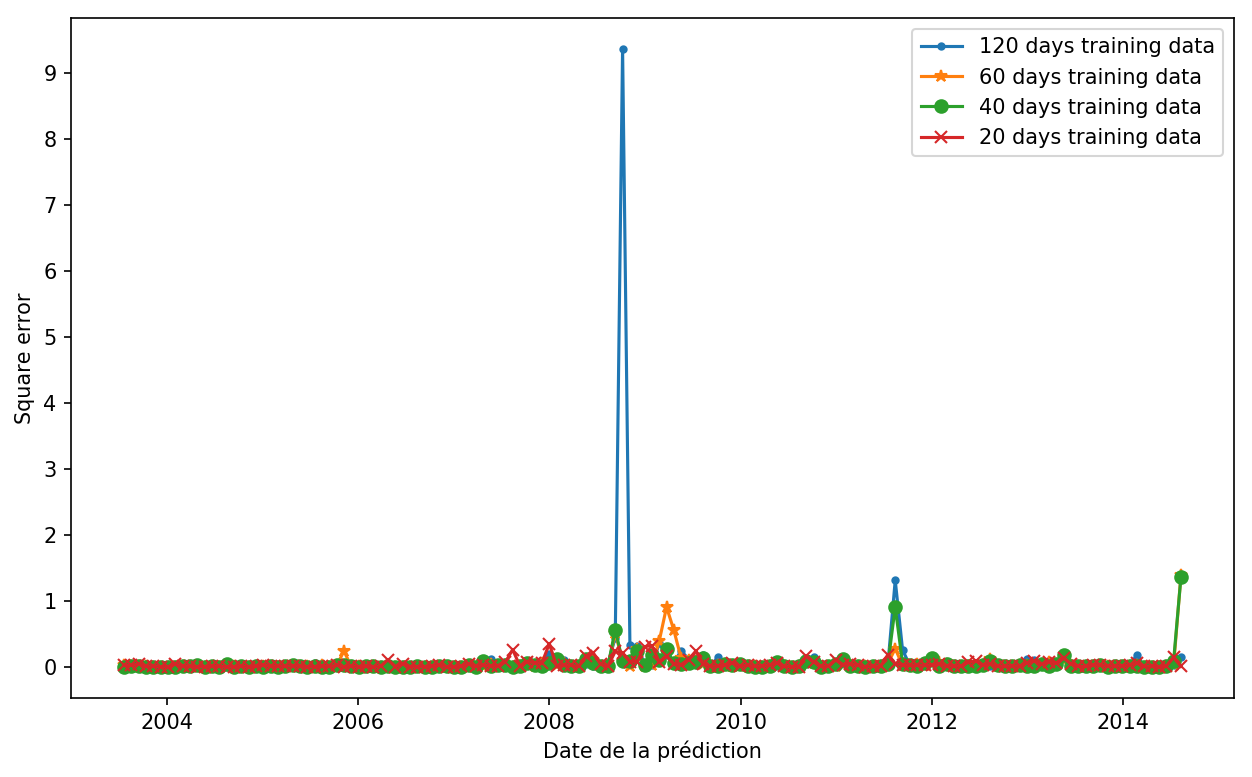
\includegraphics[width=.9\linewidth, scale=0.2]
{plot/SE_Trainingset.png}
\caption{Vue globale sur 10 ans}
\label{fig:SE_Ts1}
\end{subfigure}%
\begin{subfigure}{.5\textwidth}
\centering
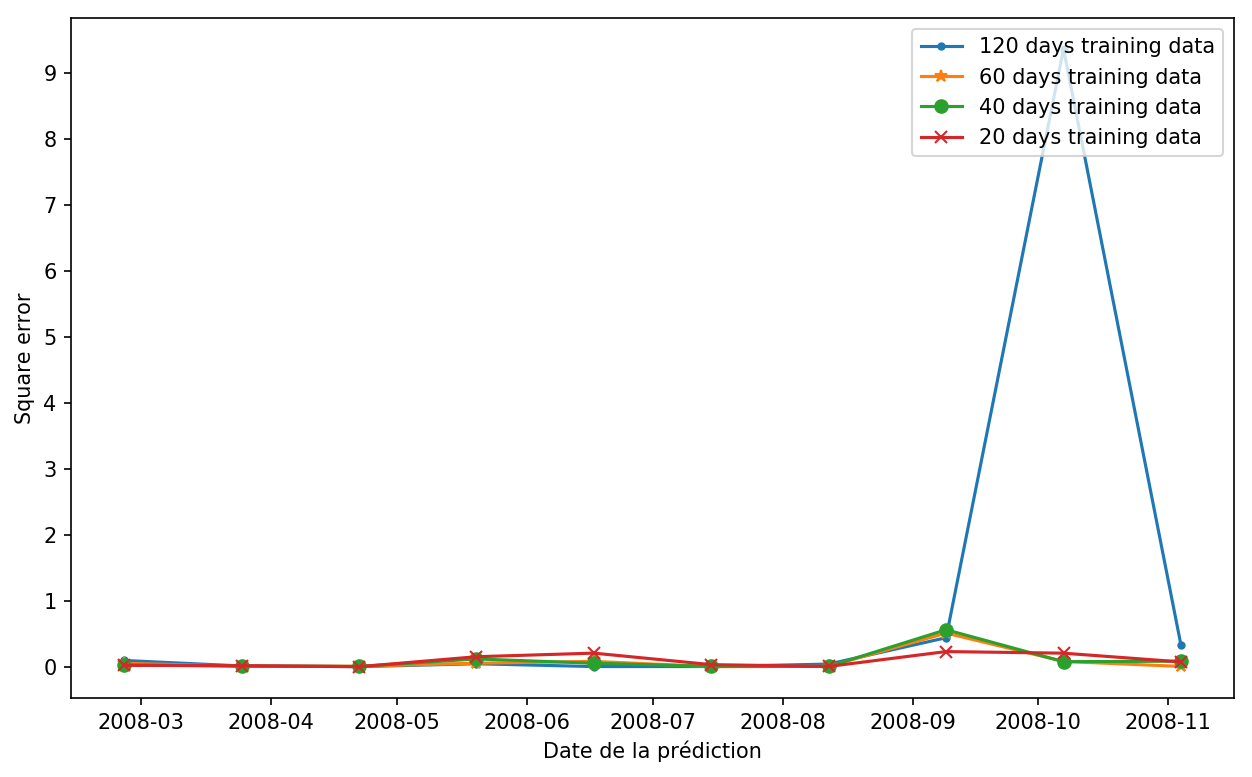
\includegraphics[width=.9\linewidth, scale=0.2]
{plot/SE_Trainingset_s.png}
\caption{Vue zoomée sur la période de la crise de 2008}
\label{fig:SE_Ts2}
\end{subfigure}
\caption{Erreur quadratique de la prédiction du rendement de Renault à un horizon de 20 jours (1 mois) en fonction de la taille d'apprentissage}
\label{fig:SE_Trainingset}
\end{figure}


\begin{figure}[H]
\centering
\begin{subfigure}{.5\textwidth}
\centering
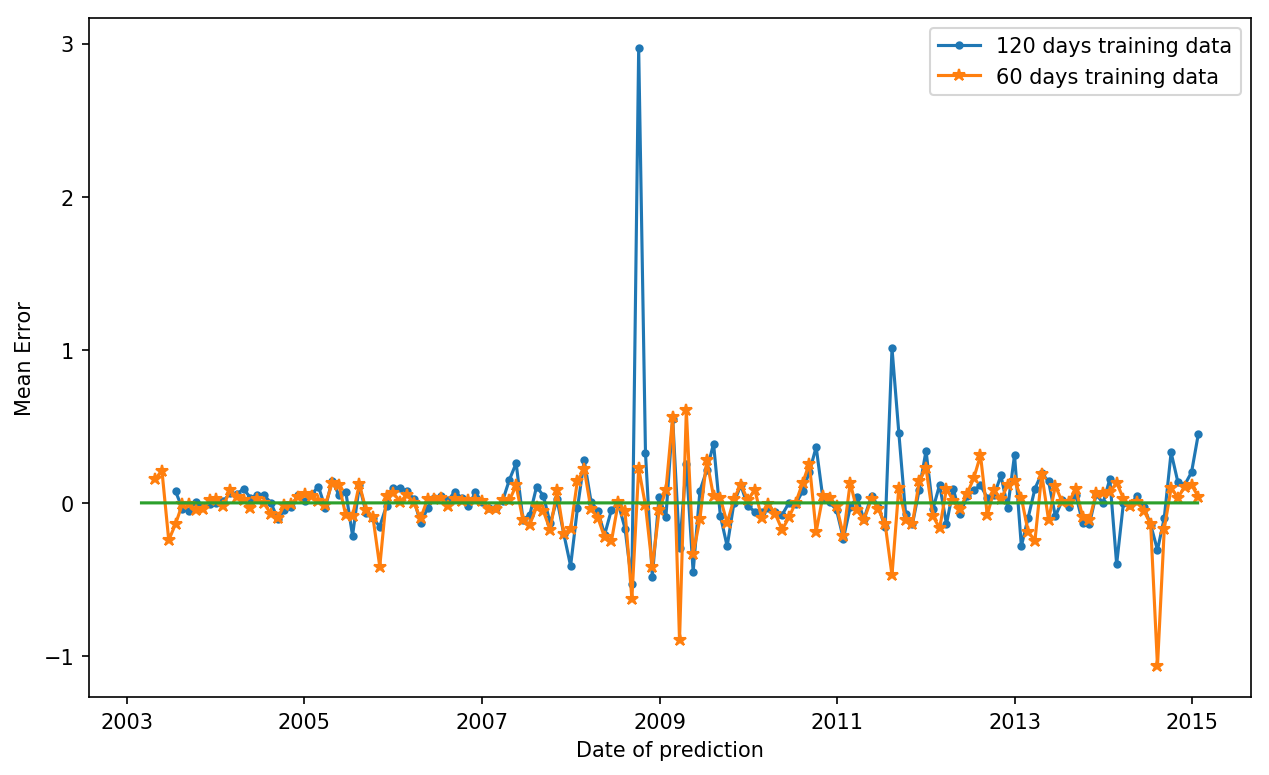
\includegraphics[width=.9\linewidth, scale=0.2]
{plot/ME_Trainingset1.png}
\caption{Erreur moyenne pour 120 et 60 jours}
\label{fig:ME_Ts1}
\end{subfigure}%
\begin{subfigure}{.5\textwidth}
\centering
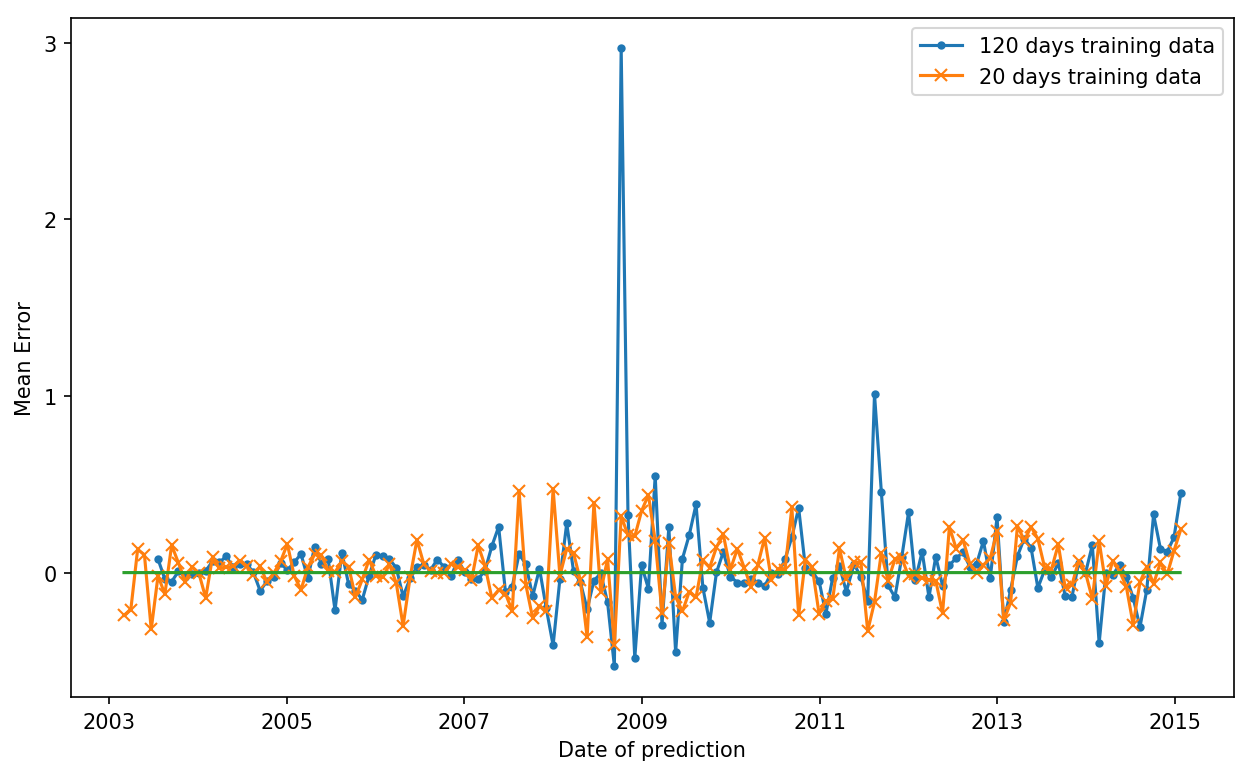
\includegraphics[width=.9\linewidth, scale=0.2]
{plot/ME_Trainingset2.png}
\caption{Erreur moyenne pour 120 et 20 jours}
\label{fig:ME_Ts2}
\end{subfigure}
\caption{Test de validation : Erreur moyenne de la prédiction du rendement de Renault à un horizon de 20 jours (1 mois) en fonction de la taille d'apprentissage}
\label{fig:ME_Trainingset}
\end{figure}


En observant la figure \ref{fig:ME_Trainingset} qui représente l'erreur moyenne de la prédiction de chaque période et la figure \ref{fig:SE_Trainingset}, nous remarquons que l'erreur moyenne pour 120 jours est généralement plus petite que les autres cas (sauf la période de la crise), car une periode plus longue contient plus d'informations et peut mieux présenter la tendance du marché. Au contraire, une période plus courte est plus bruitée. \\

Nous avons fait varier la taille d'apprentissage de cette façon également sur la base de test pour voir si les résultats sont cohérents, qui sont détaillés dans le paragraphe \ref{sec:tp} suivant.\\



\paragraph{Test de prédiction}\label{sec:tp}

Les résultats de prédiction sur la base de test sont présentés en figure \ref{fig:tp_mse}. Ils nous montrent que l'erreur quadratique de la prédiction est toujours grande autour de la crise de 2008, ainsi que la récession de 2011. C'est donc cohérent avec les résultats des tests de validation. En plus de cela, un nouveau pic appraît en 2013, puisque à ce moment là, il y avait une forte croissance du marché Automibile mondial, et que Renault a réussi à soutenir sa présence à l'international et a réalisé beaucoup plus de ventes hors Europe par rapports aux périodes précedentes.\\


\begin{figure}[H]
\centering
\begin{subfigure}{.5\textwidth}
\centering
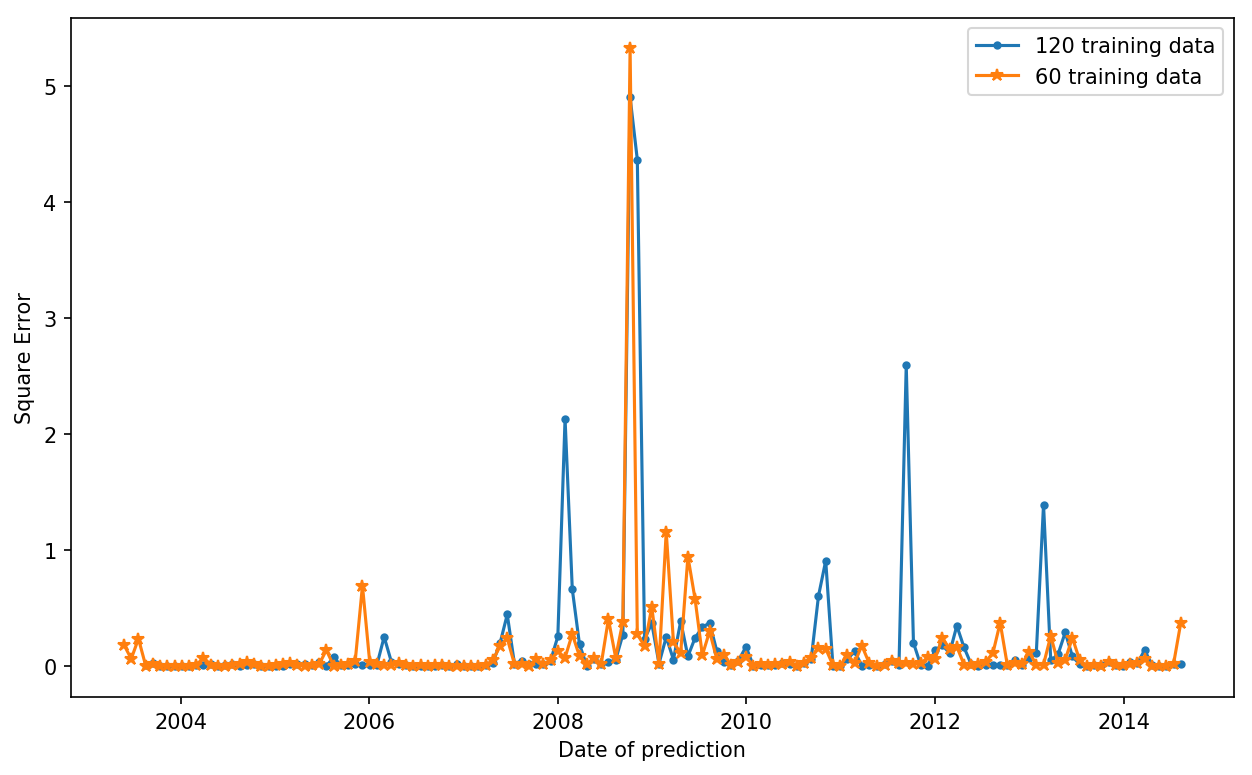
\includegraphics[width=.9\linewidth, scale=0.2]
{plot/Predict1.png}
\caption{Erreur quadratique pour 120 et 60 jours}
\label{fig:p1}
\end{subfigure}%
\begin{subfigure}{.5\textwidth}
\centering
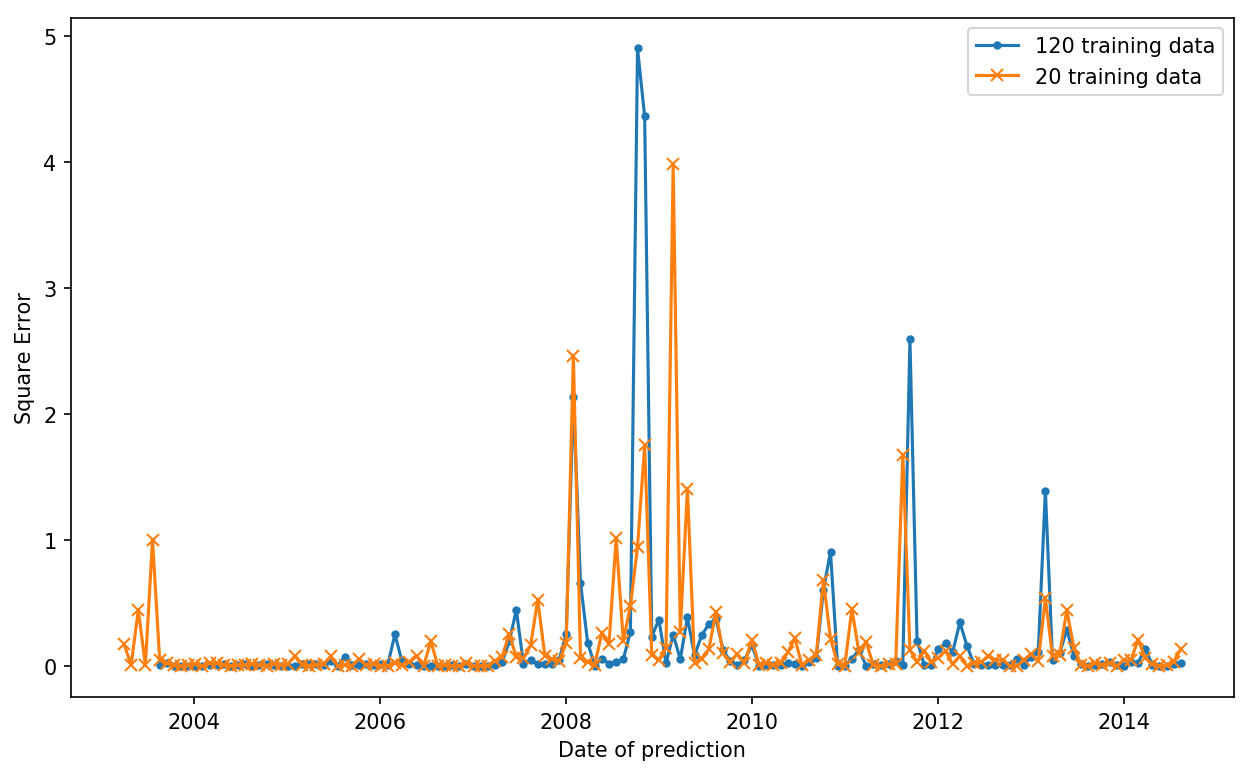
\includegraphics[width=.9\linewidth, scale=0.2]
{plot/Predict2.png}
\caption{Erreur quadratique pour 120 et 20 jours}
\label{fig:p2}
\end{subfigure}
\caption{Test de prédiction : Erreur quadratique de la prédiction du rendement de Renault à un horizon de 20 jours (1 mois) en fonction de la taille d'apprentissage}
\label{fig:tp_mse}
\end{figure}

En général, avec une base d'apprentissage de 120 jours, nous obtenons les meilleurs résultats sur des périodes calmes. Pour cette raison, nous avons réalisé des tests de prédiction avec une taille d'apprentissage égale à 120 jours, qui sont présentés dans les sections suivantes ainsi que les tests de tous les autres scénarios. Cependant, sur des périodes perturbées, la prédiction avec l'apprentissage de 60 jours offre un meilleur résultat, qui est capable de capturer plus d'informations récentes.\\

Comme indiqué en figure \ref{fig:test}, l'erreur quadratique de tests est plus grande que celle de validation, parce que la base de test est décalée de la distance temporelle d'un horizon, 20 jours dans notre cas. Il est donc plus difficile de prédire avec une base d'apprentissage qui contient que des informations de 20 jours avant.


\begin{figure}[H]
\centering
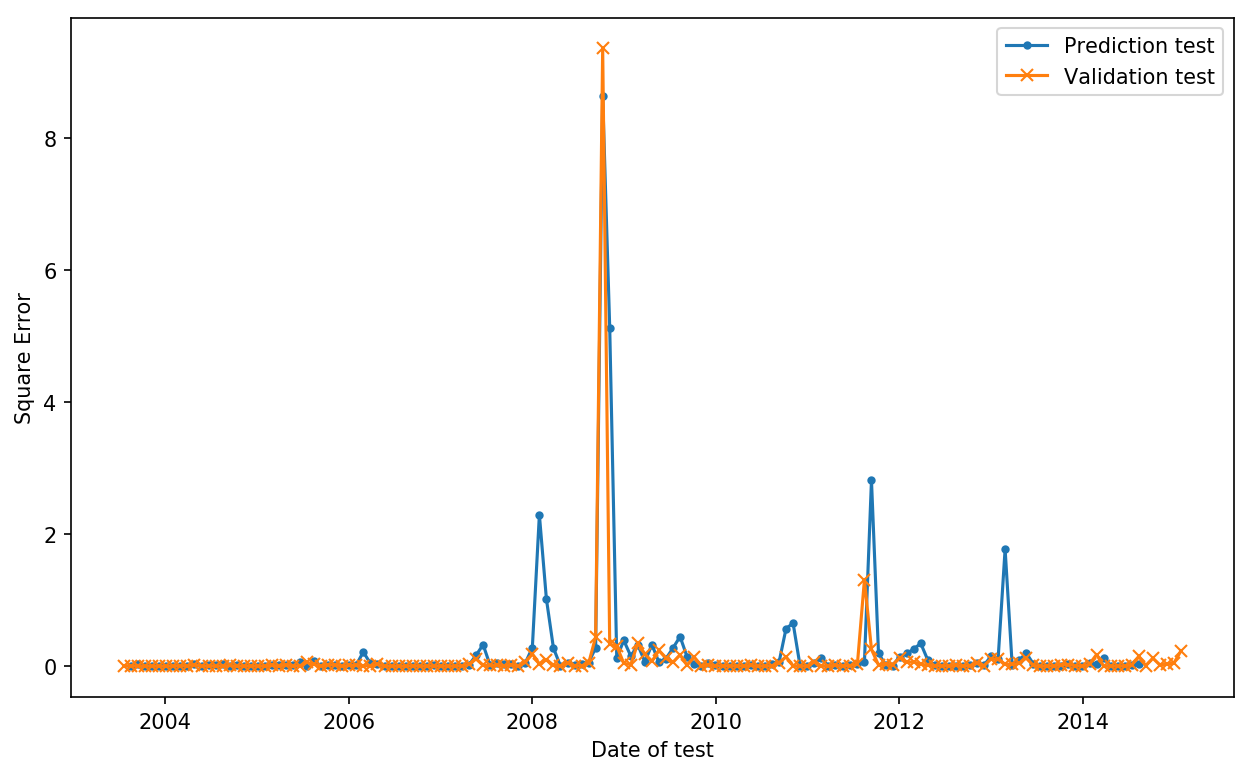
\includegraphics[width=.9\linewidth, scale=0.2]
{plot/VP.png}
\caption{Comparaison de tests de prédiction et de validation}
\label{fig:test}
\end{figure}

\subsubsection{Variation de l'horizon}

Nous discutons l'influence de l'horizon de prédiction dans cette partie, pour déterminer la fréquence de la gestion d'un portefeuille, il faut bien choisir un horizon de prédiction. Si nous prenons un horizon très court, ça va générer un coût opérationel très élevé, parce que nous avons besoin de prendre plus de temps et plus de ressources. Par contre, si nous définissons un horizon plus long, il est plus difficile de prédire la valeur très future, donc ça va dégrader la performance du modèle. \\

Nous avons fixé la taille de base d'apprentissage à 120 jours (6 mois) et la taille de base de test à 20 jours (1 mois), nous avons pris tout les 13 TIs, nous n'avons changé que l'horizon de prédiction. Nous avons préparé 6 tests pour savoir l'influence des horizons différents, nous avons varié l'horizon sur 5 jours (1 semaine), 10 jours (2 semaines), 20 jours (1 mois), 40 jours (2 mois), 60 jours (3 mois), 120 jours (6 mois). \\

\begin{figure}[H]
	\centering
	\begin{subfigure}{.5\textwidth}
	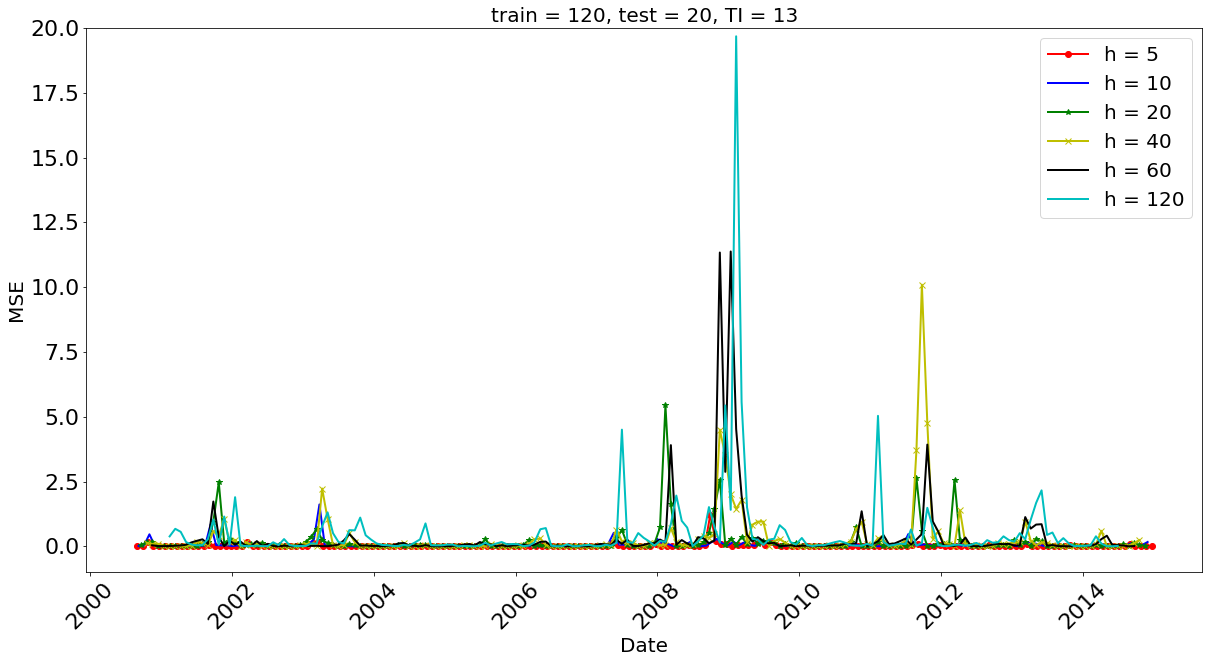
\includegraphics[width=.9\linewidth, scale=0.2]
	{plot/MSE_120_h_20.png}
	\caption{MSE en fonction de la variation de l'horizon}
	\label{fig:Horizon}
	\end{subfigure}%
	\begin{subfigure}{.5\textwidth}
	\centering
	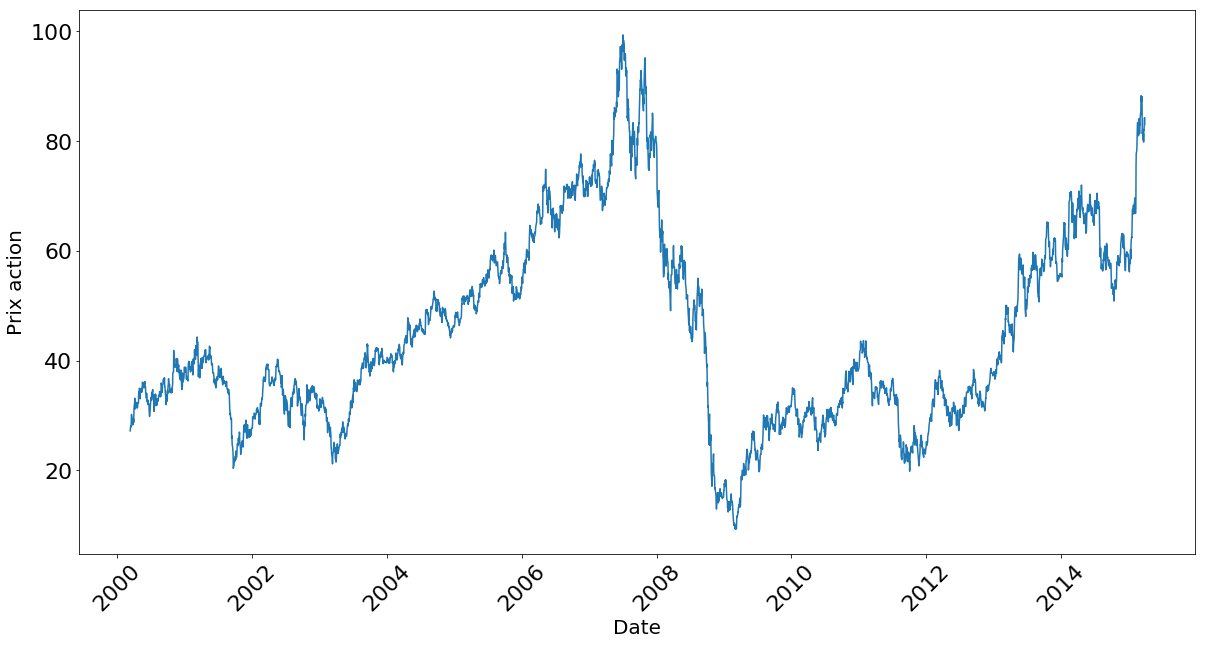
\includegraphics[width=.9\linewidth, scale=0.2]
	{plot/Prix_action_global.png}
	\caption{Evolution du Prix d'action Renault}
	\label{fig:Prix_action}
	\end{subfigure}
\caption{Influence de l'horizon sur en vue globale pendant 2000 - 2015}
\label{fig:Horizon_global}
\end{figure}

Nous pouvons obtenir le résultat global sur 15 ans dans la figure \ref{fig:Horizon}. Suivi l'augementation de l'horizon, nous pouvons constater que la prériode défavorable est plus fluctuante et il y a plus de pics sur la courbe. Pendant la période stable, les erreurs moyennes quadratiques sont plus proche de zéro quand l'horizon est plus petit. En comparant avec l'évolution du prix d'action Renault, nous avons trouvé que quand il y a une baisse évidente, les erreure de prédictions sont aussi plus grandes. \\

Sur la figure \ref{fig:Prix_action}, il y a 5 baisses plus évidentes sur la courbe, elles sont dans le septembre 2001, le mars 2003, le septembre 2008, l'octobre 2011 et le novembre 2014. Nous avons fait des recherches pour expliquer les baisses du cours. A la suite des événements du 11 septembre 2001, Renault atteint le 21 septembre son point bas de l'année à 26,01 euros.\footnote{Rapport annuel d’activité
Renault 2001} Le titre Renault connaît un plus bas le 12 mars 2003 à 29,51 euros, suivant le mouvement de baisse du secteur automobile, pénalisé par les incertitudes économiques et géopolitiques et affecté par le recul des performances commerciales du début d’année.\footnote{Rapport annuel d’activité
Renault 2003} Le septembre 2008 est la crise financière mondiale, le prix d'action de Renault a été beaucoup influencé. Comme nous avons dit dans la section précédente, il y a une recession dans l'année 2011. Renault a accusé une baisse globale de 5 pourcents de ses ventes en novembre 2014. \footnote{Rapport annuel d’activité Renault 2014} Pendant ces périodes défavorables, la situstion est plus pire, les erreurs de prédictions sont plus grandes. Quand l'horizon est plus long, la courbe est plus perturpée. \\ 


Pour comparer l'impact de l'horizon sur les périodes différentes, nous avons aussi fait un zoom sur la période autour de la crise financière de 2008, les figures ci-après vous montre nos résultat. La figure \ref{fig:Prix_crise} est le prix d'action entre 2007 et 2010, nous pouvons trouver qu'à partir du septembre 2007, la courbe commence à baisser progressivement et elle apparait une chute au septembre 2008. Après mars 2009, le prix d'action commence à revenir. La figure \ref{fig:Horizon_crise} nous montre que pendant la crise toutes les prédictions ne sont pas stables, il y a des grandes erreurs de prédiction sur chaque courbe. Par contre, quand l'horizon est plus long, il y a un retard de détection sur la tendance de baisse. Quand l'horizon est 20, ses pics sont plus proche au début de la baisse de cours, pour l'horizon est égale à 60 et 120, il y a toujours un grand décalage avec la date début. Les figures \ref{fig:Horizon_before} et \ref{fig:Horizon_after} sont les prériodes avant et après la crise de 2008, nous pouvons consatater que les erreurs sont négligables par rapports à la prériode de crise. Mais, l'horizon est plus grand, la courbe est plus fluctuante.

\begin{figure}[H]
	\centering
	\begin{subfigure}{.5\textwidth}
	\centering
	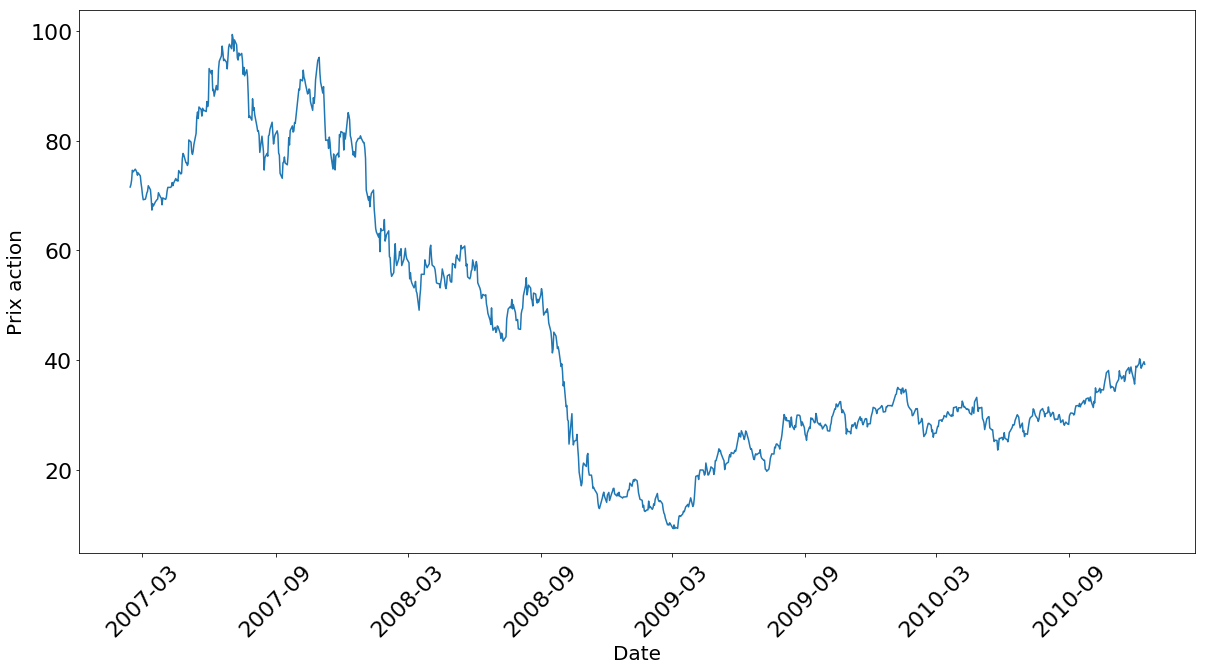
\includegraphics[width=.9\linewidth, scale=0.2]
	{plot/Prix_action_crise.png}
	\caption{Prix d'action pendant la crise 2008}
	\label{fig:Prix_crise}
	\end{subfigure}%
	\begin{subfigure}{.5\textwidth}
	\centering
	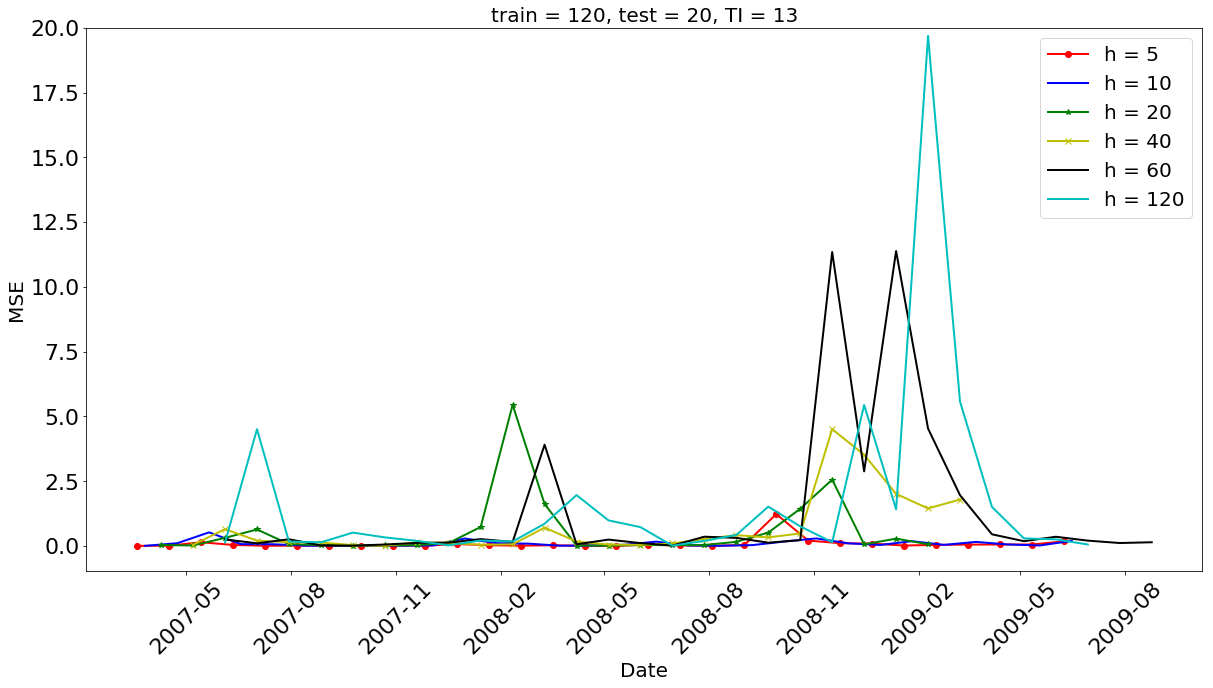
\includegraphics[width=.9\linewidth, scale=0.2]
	{plot/MSE_120_h_20_crise.png}
	\caption{MSE pendant la crise 2008}
	\label{fig:Horizon_crise}
	\end{subfigure} 
	\begin{subfigure}{.5\textwidth}
	\centering
	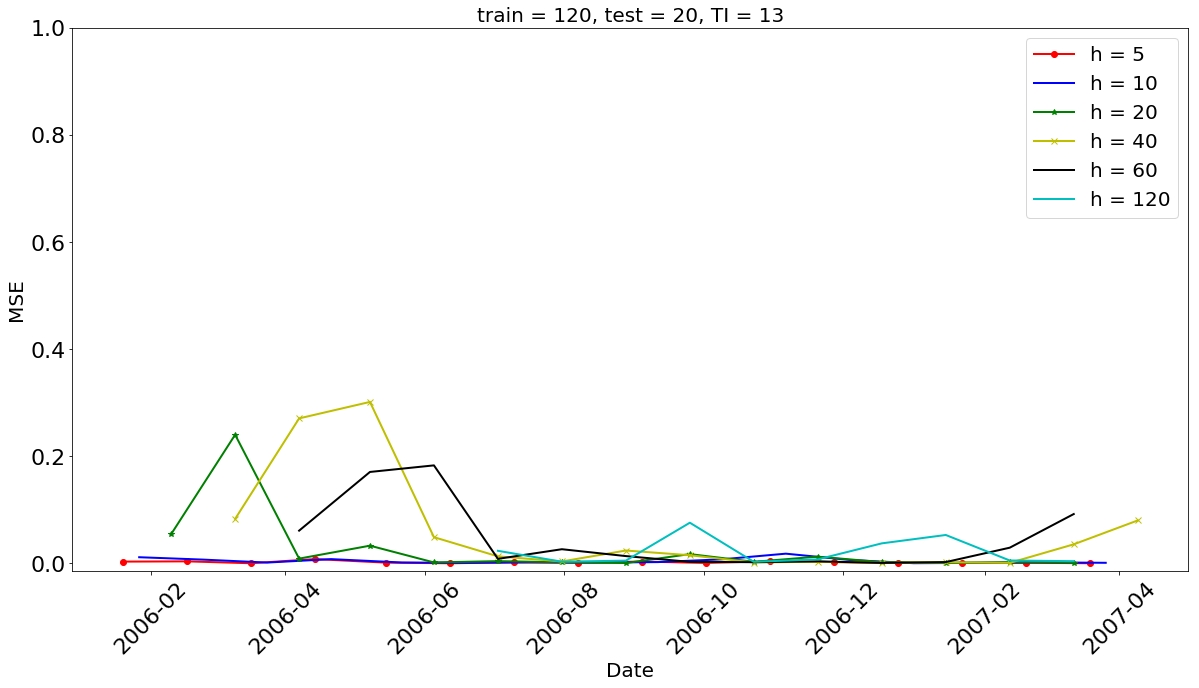
\includegraphics[width=.9\linewidth, scale=0.2]
	{plot/MSE_120_h_20_before.png}
	\caption{MSE avant la crise 2008}
	\label{fig:Horizon_before}
	\end{subfigure}%
	\begin{subfigure}{.5\textwidth}
	\centering
	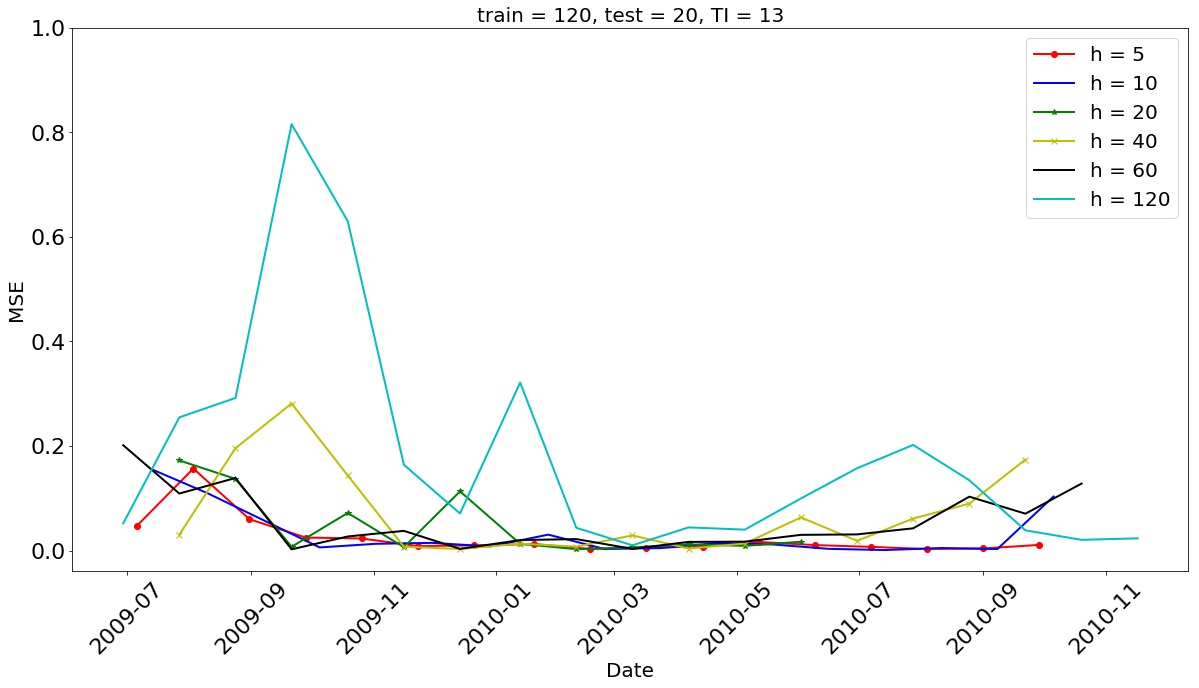
\includegraphics[width=.9\linewidth, scale=0.2]
	{plot/MSE_120_h_20_after.png}
	\caption{MSE après la crise 2008}
	\label{fig:Horizon_after}
	\end{subfigure}
\caption{Influence de l'horizon sur les prériodes différentes}
\label{fig:MSE_horizon}
\end{figure}

Nous avons choisi 20 jours comme l'horizon du rendement, parce que les erreurs moyennes quadratiques de 5, 10 et 20 jours sont relativement faibles par rapport aux celles de 60 et 120 jours, ainsi il n'y a pas trop de retard entre la valeur de prédiction et la vraie valeur. En comparant avec 5 et 10 jours, son courbe n'a pas beaucoup de changement et aussi l'horizon de 20 est plus faisable dans la réalité. Par conséquent, nous prenons l'horizon de 20 jours dans les autres scénarios de test.

\subsubsection{Variation de taille de test}

Nous voudrons savoir l'effet de la durée de test, donc nous lançons ce scénario de test pour trouver une taille idéal. Dans les deux scénarios précédents, nous avons fixé la taille de base d'apprentissage à 120 jours et l'horizon de prédiction est 20 jours. Nous les avons gardé dans cette partie, ainsi les 13 TIs. Nous n'avons joué que sur la durée de test, nous avons testé sur 5 jour, 20 jours, 60 jours et 120 jours. \\ 

Nous pouvons constatons que plus la taille de test est petite, plus de pics se trouvent dans la courbe de l'erreur. Dans la figure \ref{fig:test_g}, nous trouvons que la courbe de test sur 60 jours est beaucoup plus glissante que les autres courbes et le test sur 5 jours varie plus fréquemment. Par conséquent, nous avons zoomé la date autour de 2008, suivi l'augmentation de la base de test, il y a moindre variation sur l'erreur et chaque pic se tient plus long temps.  \\

\begin{figure}[H]
	\centering
	\begin{subfigure}{.5\textwidth}
	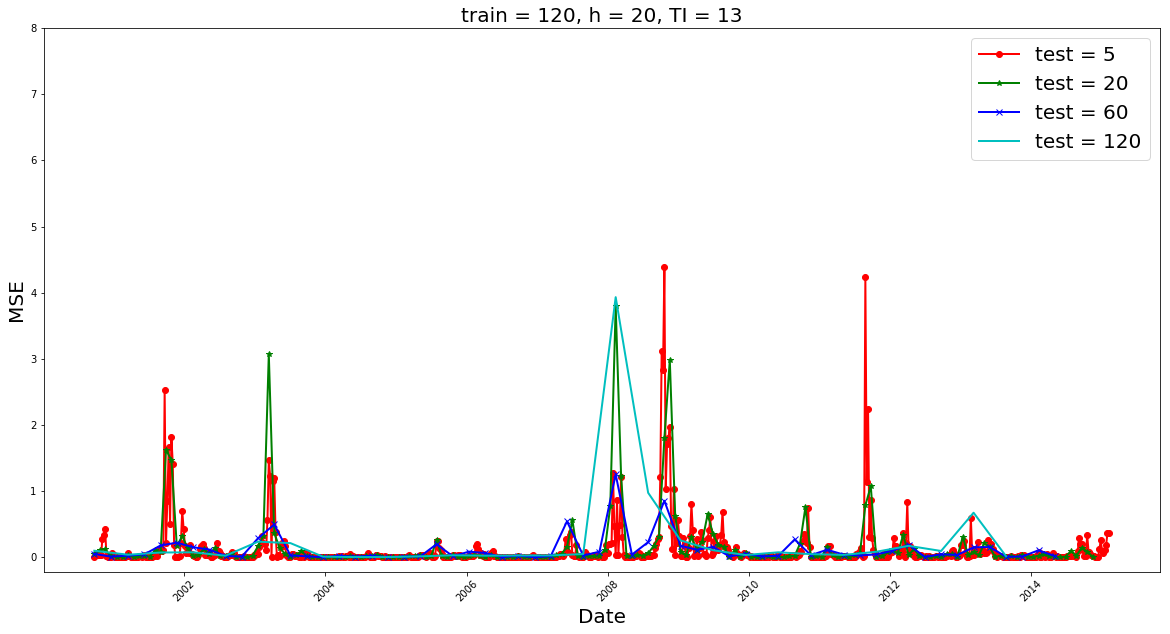
\includegraphics[width=.9\linewidth, scale=0.2]
	{plot/MSE_test_global.png}
	\caption{MSE sur la variation de durée de test en vue global}
	\label{fig:test_g}
	\end{subfigure}%
	\begin{subfigure}{.5\textwidth}
	\centering
	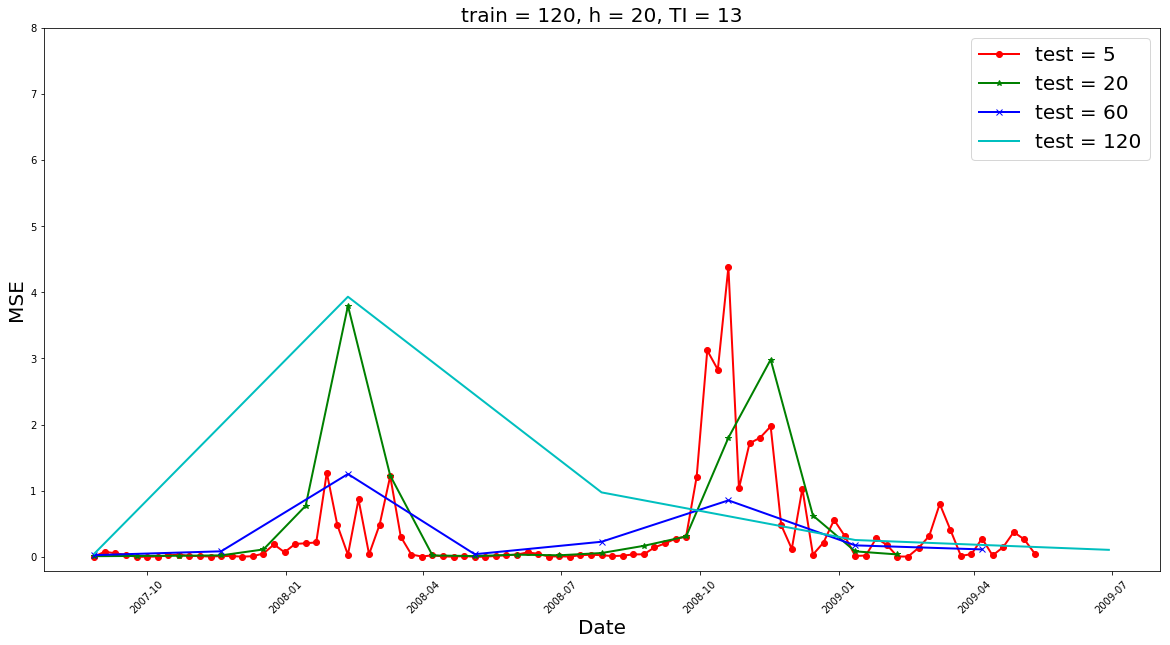
\includegraphics[width=.9\linewidth, scale=0.2]
	{plot/MSE_test_2008.png}
	\caption{MSE sur la variation de test pendant la crise 2008}
	\label{fig:test_2008}
	\end{subfigure}
\caption{Influence de la durée de test sur en vue globale pendant 2000 - 2015}
\label{fig:MSE_test}
\end{figure}

Comme nous voudrons un modèle plus stable, nous ne pouvons pas prender une taille de test trop courte ayant les résultats désorganisés. Cependant, si nous choisissons une base de test très grande, nous aurons des erreurs plus élevées. Par conséquent, nous avons fixer 20 jours pour la base de test, et nous les avons aussi appliqué aux autres scénarios de test.



\subsubsection{Variation de nombre de TIs}

Les TIs calculés à partir des données historiques se situent dans 4 catégories qui peuvent décrire le mouvement du marché financier par des façons différentes. Dans ce scénario de test, nous voudrons savoir si on peut utiliser moindre TIs pour obtenir une meilleur performance. \\

Nous avons d'abord calculer la corrélation entre les 13 TIs pour savoir qu'il y a combien de TIs est redundant. La figure \ref{fig:corr} vous donne une vue synthétique sur la corrélation entre les 13 TIs, la couleur plus claire représente une corrélation plus haute. Nous n'avons affiché que les TIs apportés une corrélation superieur à 90 pourcents dans la figure \ref{fig:corr_s}. Nous pouvons trouver que l'indicateur SMA et EMA ont une forte corrélation, donc nous décidons d'éliminer un des deux indicateurs. \\

\begin{figure}[H]
	\centering
	\begin{subfigure}{.5\textwidth}
	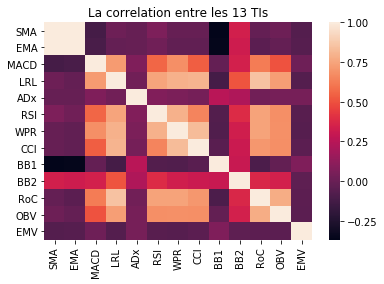
\includegraphics[width=.9\linewidth, scale=0.2]
	{plot/Corr.png}
	\caption{Représentation visualisée pour la corrélation}
	\label{fig:corr}
	\end{subfigure}%
	\begin{subfigure}{.5\textwidth}
	\centering
	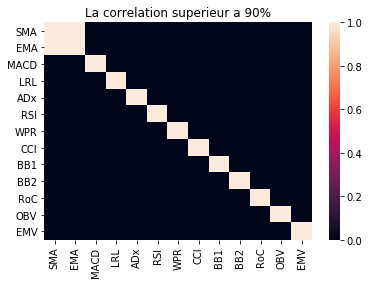
\includegraphics[width=.9\linewidth, scale=0.2]
	{plot/corr_s.png}
	\caption{Corrélation superieur à 0.9}
	\label{fig:corr_s}
	\end{subfigure}
\caption{Corrélation entre les 13 TIs}
\label{fig:correlation}
\end{figure}

Comme les tests précédents, nous avons pris une taille de base d'apprentissage à 120 jours (6 mois), la taille de base de test à 20 jours (1 mois), et l'horizon de prédiction est 20 jours (1 mois). Cette fois, nous ne varions que sur le nombre de TIs, nous avons fait 3 tests sur ce scénario. Nous prenons tous les 13 TIs comme le premier test, et puis nous supprimons l'indicateur EMA pour tester les autres 12 TIs. A la fin, nous tirons 4 indicateurs par catégorie, soit SMA,CCI,BB1,EMV. \\

La figure \ref{fig:TI} vous montre le résltat de test du changement de TIs, selon ce graphique, nous consatons que les trois courbes ont presque le même comportement en vue globale, c'est-à-dire qu'elles sont plus perturbées pendant les périodes défavorables et plus stables dans les périodes calmes. Cependant, nous pouvons trouver que la courbe de 4 indicateurs est plus sensible aux baisses de 2001 et 2003, et les courbes de 13 et 12 indicateurs sont plus sensibles à la crise de 2008. 

\begin{figure}[H]
	\centering
	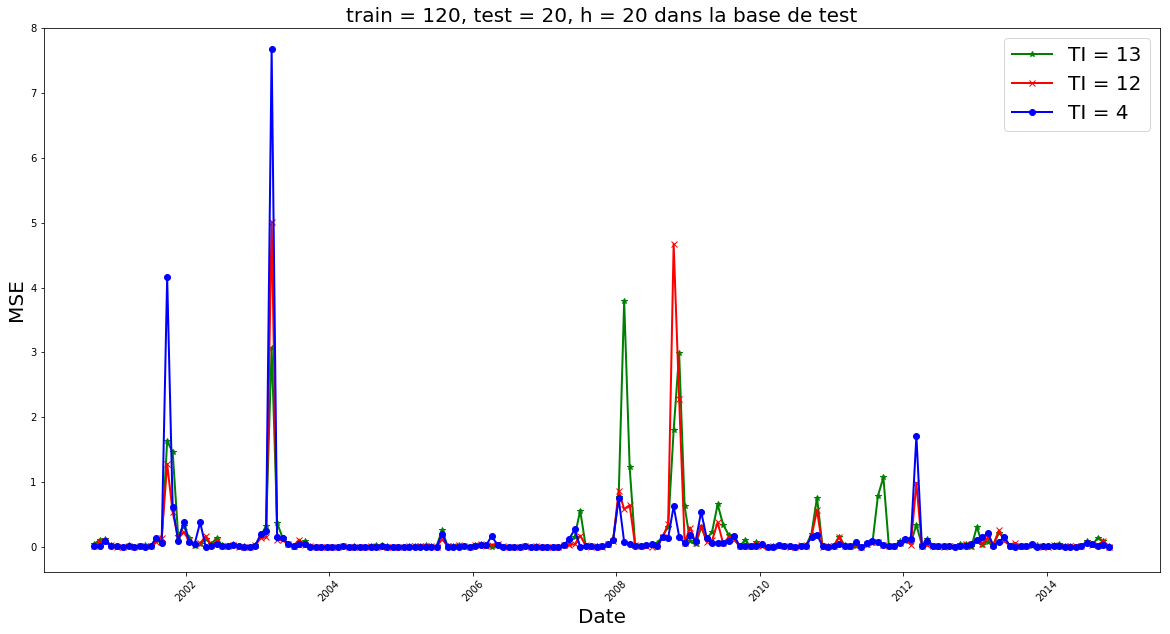
\includegraphics[width=.9\linewidth, scale=0.2]
	{plot/MSE_120_20_20_N_test.png}
	\caption{MSE en fonction de la variation de TIs en vue global dans la base d'apprentissage}
	\label{fig:TI}
\end{figure}



\begin{figure}[H]
	\centering
	\begin{subfigure}{.5\textwidth}
	\centering
	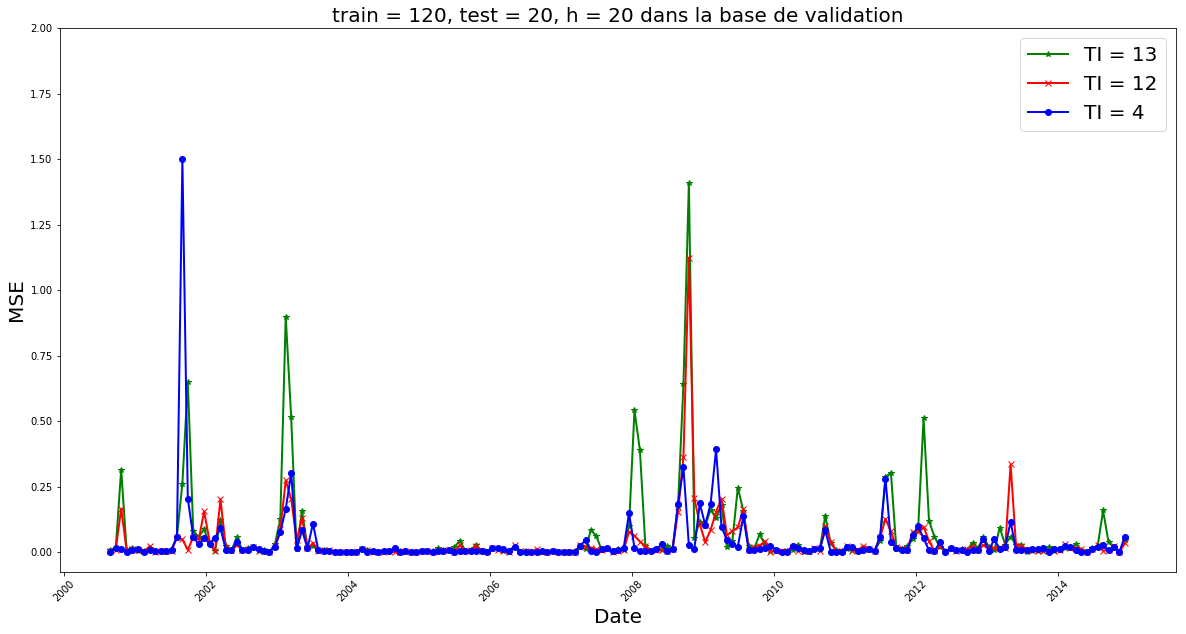
\includegraphics[width=.9\linewidth, scale=0.2]
	{plot/MSE_120_20_20_N_val.png}
	\caption{Comparaison en vue globale dans la base de test}
	\label{fig:val_test_13}
	\end{subfigure}%	
	\begin{subfigure}{.5\textwidth}
	\centering
	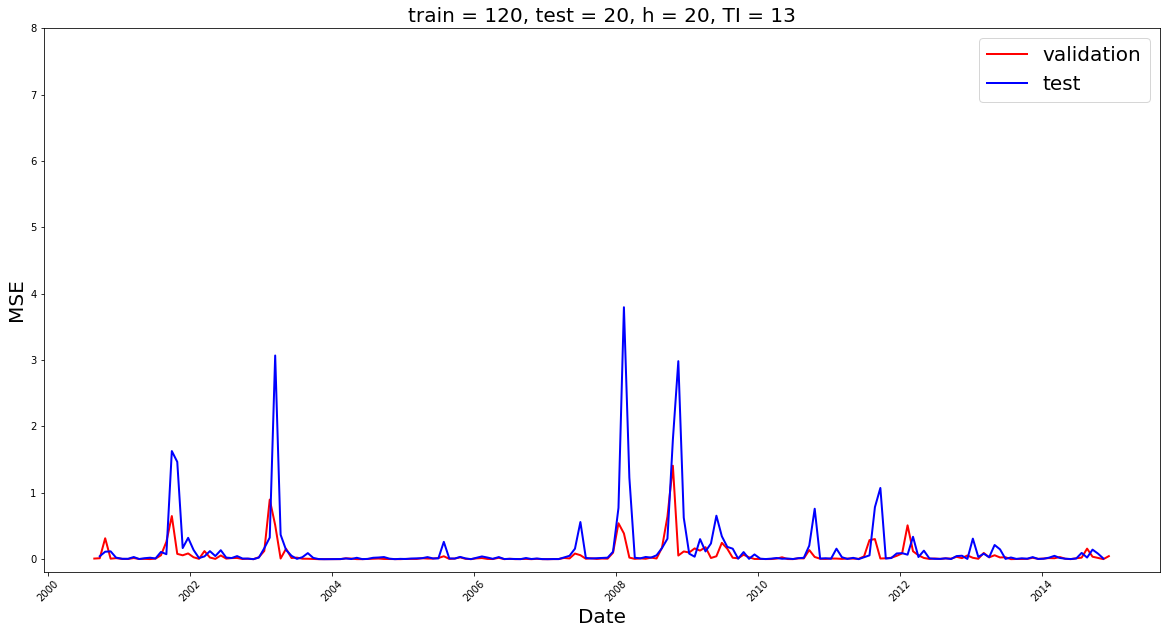
\includegraphics[width=.9\linewidth, scale=0.2]
	{plot/val_test_120_20_20_13.png}
	\caption{Comparaison avec 13 TIs}
	\label{fig:val_test_13}
	\end{subfigure}
	\begin{subfigure}{.5\textwidth}
	\centering
	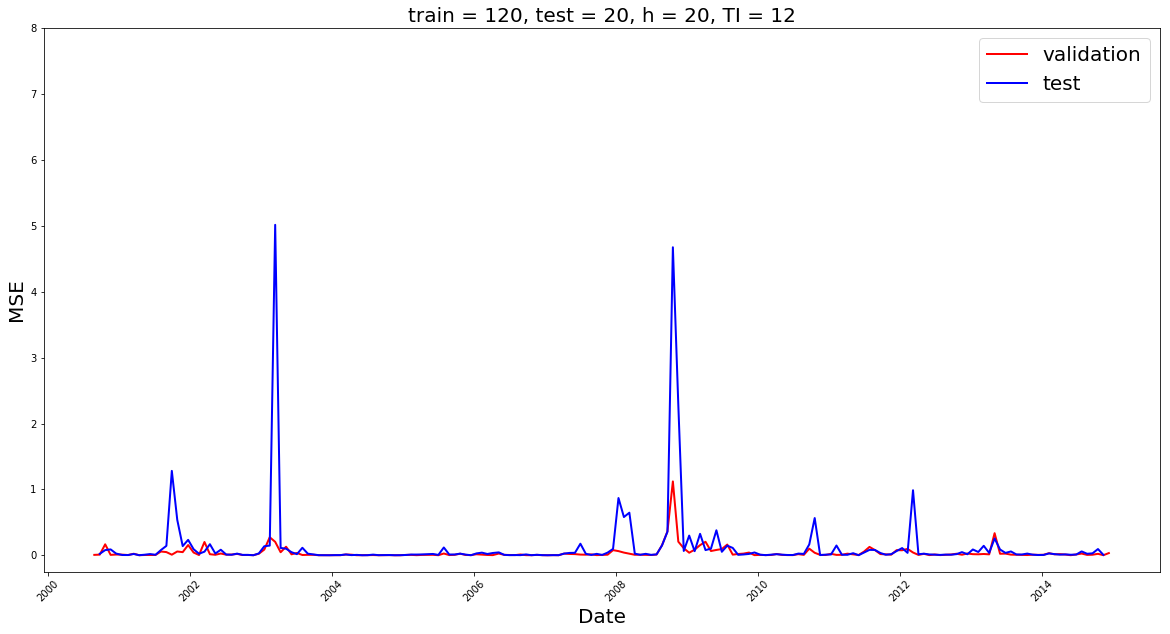
\includegraphics[width=.9\linewidth, scale=0.2]
	{plot/val_test_120_20_20_12.png}
	\caption{Comparaison avec 12 TIs}
	\label{fig:val_test_12}
	\end{subfigure}%
	\begin{subfigure}{.5\textwidth}
	\centering
	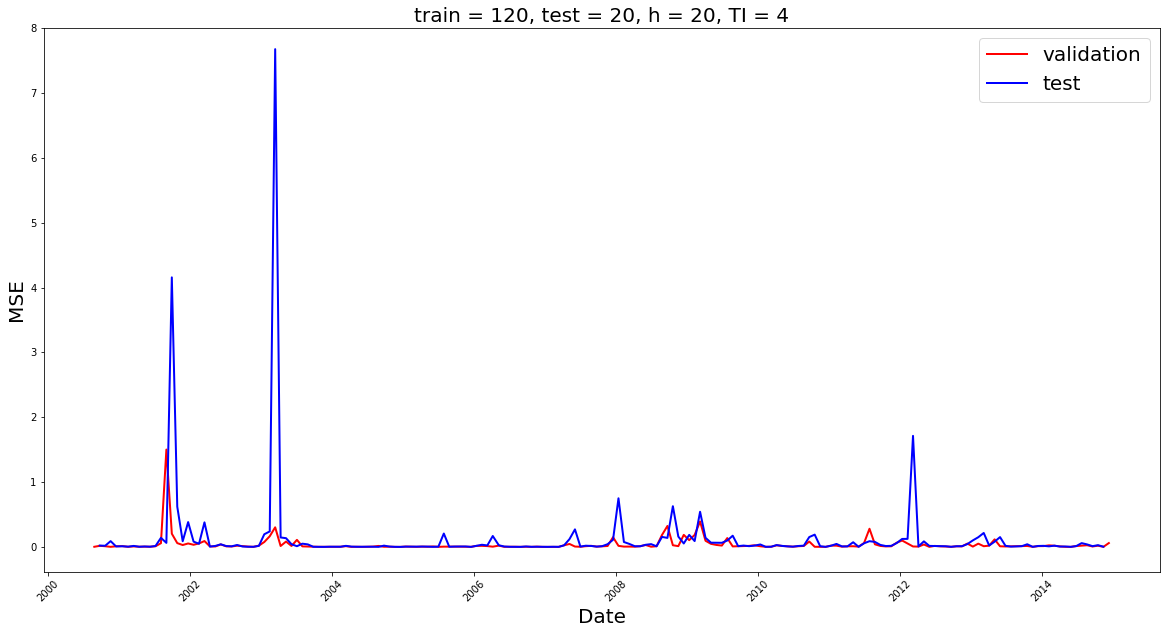
\includegraphics[width=.9\linewidth, scale=0.2]
	{plot/val_test_120_20_20_4.png}
	\caption{Comparaison avec 4 TIs}
	\label{fig:val_test_4}
	\end{subfigure}	
\caption{Comparaison entre la base d'apprentissage et de test}
\label{fig:val_test_TI}
\end{figure}

Nous avons aussi fait un test dans la base d'apprentissage, la figure \ref{fig:val_test_TI} donne les erreurs dans la base de validation et la comparaison entre les deux bases. Nous pouvons trouver que l'amplitude de la courbe en vue globale sur la base de validation est plus petite que celle dans la base de test. Et puis, nous avons aussi fait une comparaison en utilisant le même nombre de TIs dans les deux bases, nous pouvons constater que les pics apparaitrent dans presque les mêmes endroites, mais leur amplitude est complètement différente.




